\chapter{Accretion and Winds}
\label{cha:accretion-winds}
We continue looking at steady flows with two specific applications:
matter flowing onto an object (accretion) and matter flowing away from
an object (winds). 

\section{Spherical Accretion}
\label{sec:spherical-accretion}
\index{fluid mechanics!spherical accretion}
\index{spherical accretion}
We can apply what we learned about the de Laval nozzle to accretion
onto an astrophysical object.  We will assume that the accretion is
steady at a rate ${\dot M}$ and that the pressure $P \propto
\rho^\gamma$ with $1 < \gamma < 5/3$.   First let's write the
continuity equation
\begin{equation}
\frac{1}{r^2} \pp{}{r} \left ( r^2 \rho v \right ) = 0 
\label{eq:718}
\end{equation}
so $\rho v r^2=$constant.  Let's write down the Euler equation
\begin{equation}
v\pp{v}{r} + \frac{1}{\rho} \pp{p}{r} + \frac{GM}{r^2} = 0
\label{eq:719}
\end{equation}
Let's use the equation of state to eliminate $p$ from the Euler
equation and use the continuity equation to eliminate $\rho$,
\begin{equation}
\frac{1}{\rho} \pp{\rho}{r} = -\frac{1}{vr^2}
\pp{}{r}(vr^2)~\rmmat{and}~\pp{p}{r} = \pp{p}{\rho} \pp{\rho}{r} =
c_s^2 \pp{\rho}{r},
\label{eq:720}
\end{equation}
we get
\begin{equation}
v\pp{v}{r} - \frac{c_s^2}{vr^2} \pp{}{r} (vr^2) + \frac{GM}{r^2} = 0.
\label{eq:721}
\end{equation}
We can rearrange this 
\begin{equation}
\frac{1}{2} \left ( 1 - \frac{c_s^2}{v^2} \right ) \pp{v^2}{r} =
-\frac{GM}{r^2} \left ( 1 - \frac{2c_s^2 r}{GM} \right ).
\label{eq:722}
\end{equation}
Far away from the star, the sound speed $c_s$ approaches some constant
value, so the right hand side of the equation will be positive at
large $r$.  We would like the gas to accelerate toward the star, so
$\pp{v^2}{r} < 0$ at large distances.  For this to be the case $v<c_s$
far from the star.   As the gas falls toward the star, it accelerates
until it reaches the critical radius.
\begin{equation}
\frac{2c_s^2 r_c}{GM} = 1
\ee 
If we use $c_s^2 = \gamma p/\rho=\gamma k T$ we get
\begin{equation}
r_c = \frac{GM}{2c_s^2(r_c)} \approx 7.5 \times 10^{13} \left (
\frac{T}{10^4 K} \right )^{-1} \left ( \frac{M}{\rmmat{M}_\odot}
\right )\rmmat{cm} 
\label{eq:723}
\end{equation}
that is much larger that most stars, so we have to worry about what
happens with $r_c$.  If the flow is subsonic when it gets to $r_c$ it
will decelerate within $r_c$ and the accretion stagnates.  If the flow
becomes supersonic before reaching $r_c$, then $\pp{v^2}{r}$ diverges
as the flow becomes supersonic.  This is unphysical because you get
two values of $v^2$ at a single value of $r$.

The only viable accretion mode is for the flow to become supersonic
precisely at $r_c$.  It then accelerates for $r<r_c$ as well.  We can
work further to determine the flow by integrating Eq.~\ref{eq:719} to get a
Bernoulli equation
\begin{equation}
\frac{v^2}{2} + \frac{c_s^2}{\gamma - 1} - \frac{G M}{r} = \rmmat{constant}
\label{eq:724}
\end{equation}
We know that as $r \rightarrow \infty$, $v^2 \rightarrow 0$ so we have
\begin{equation}
\frac{v^2}{2} + \frac{c_s^2 - c_s^2(\infty)}{\gamma - 1} - \frac{G M}{r} = 0.
\label{eq:725}
\end{equation}
At the critical radius we have $v^2=c_s^2$ and $GM/r_c = 2 c_s^2$, so
\begin{equation}
\frac{c_s^2(r_c)}{2} + \frac{c_s^2(r_c) - c_s^2(\infty)}{\gamma-1} - 2
c_s^2(r_c) = 0 .
\label{eq:726}
\end{equation}
We can find that
\begin{equation}
c_s^2(r_c) = c_s^2(\infty) \left [ \frac{2}{5 - 3 \gamma } \right ]
\label{eq:727}
\end{equation}
so
\begin{equation}
r_c = \frac{G M}{c_s^2(\infty)} \frac{5 - 3 \gamma}{4}
\label{eq:728}
\end{equation}
and
\begin{equation}
\rho (r_c) = \rho(\infty) \left [ \frac{2}{5-3\gamma} \right ]^{1/(\gamma-1)}
\label{eq:729}
\end{equation}
We can determine 
\begin{eqnarray}
{\dot M} &=& 4\pi r_c^2 \rho(r_c) c_s(r_c) = \pi G^2 M^2
\frac{\rho(\infty)}{c_s^3(\infty)} \left(  \frac{2}{5-3\gamma} \right
)^{(5-3\gamma)/2(\gamma-1)} \\
&=& 1.4 \times 10^{11}\rmmat{g s}^{-1} \left
(\frac{M}{\rmmat{M}_\odot} \right )^2 \left [
  \frac{\rho(\infty)}{10^{-24} \rmmat{g cm}^{-3}} \right ] \left [
  \frac{c_s(\infty)}{10 \rmmat{km s}^{-1}} \right ]^{-3}.
\label{eq:730}
\end{eqnarray}
for $\gamma=1.4$.  The gamma-dependent factor ranges from $e^{3/2}$
for $\gamma=1$, to $5/2$ at $\gamma=7/5$ and 1 at $\gamma=5/3$.
{
\begin{figure}
\centering
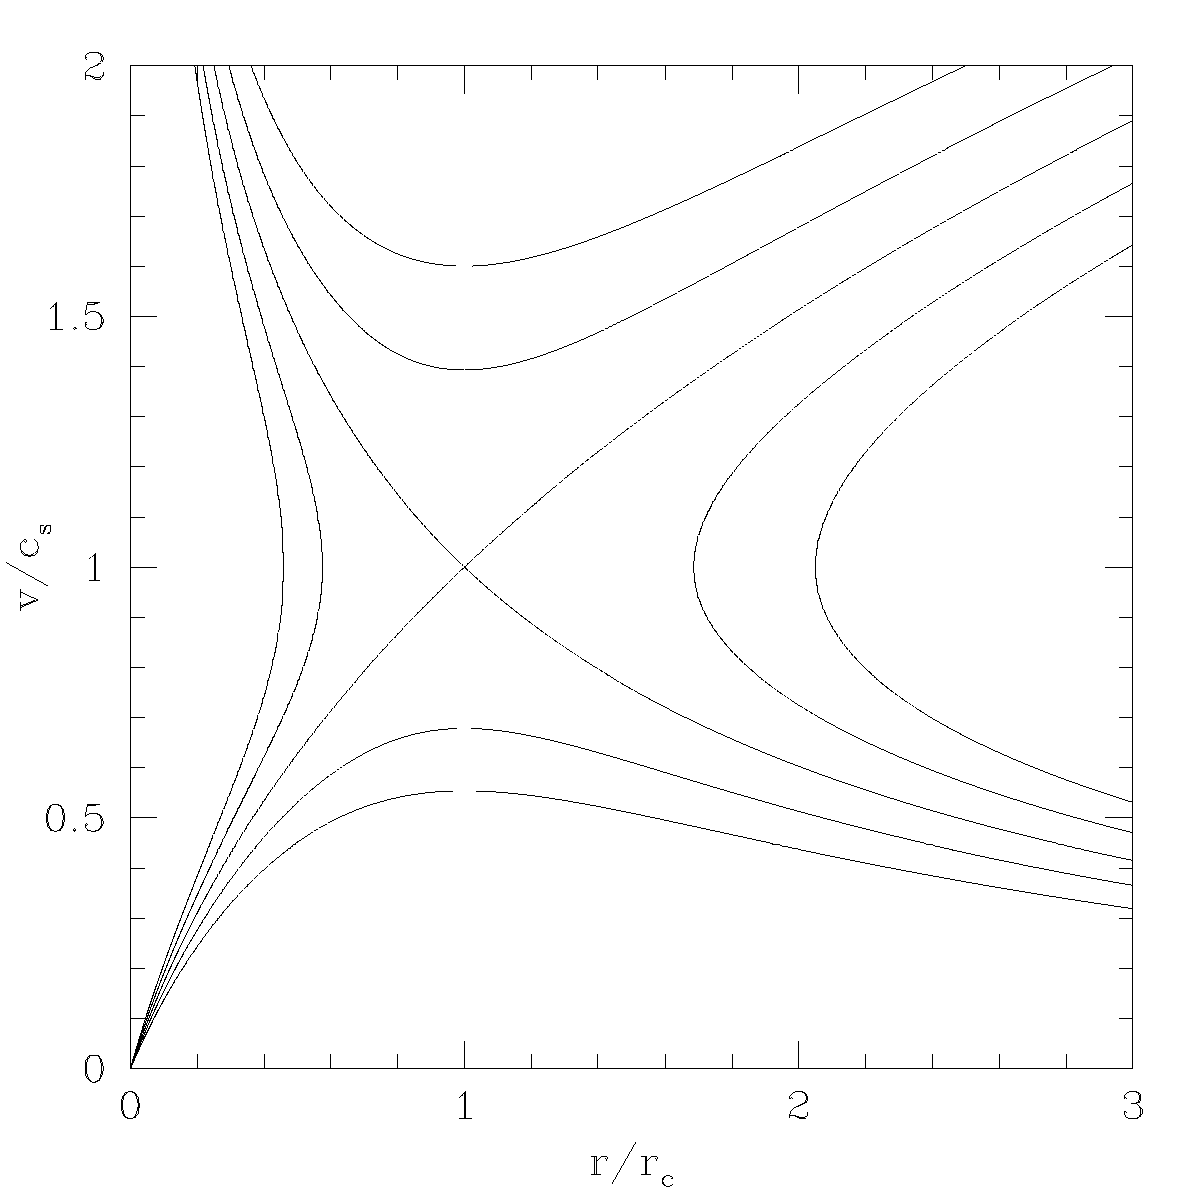
\includegraphics[width=\textwidth]{bondijsh} 
\caption{The solution to Bondi accretion with $\gamma=7/5$ (an
  adiabatic, diatomic gas).}
\label{fig:bondi}
\end{figure}
}

\section{Accretion Disks}
\index{fluid mechanics!accretion disks}
\index{accretion disks}

The preceding section ignores an important aspect of accretion: the
angular momentum of the accreta.  If the material starts with some net
angular momentum it can only collapse so far before its angular
velocity will be sufficient to halt further collapse.  For the
accetion to proceed, angular momentum must be transferred outwards
through the accreted material or removed from the central regions with
ejecta.  Understanding the production of ejecta is beyond our scope, but
examining the transport of angular momentum through a rotating disk of
material is not once we add an additional ingredient to our analysis, 
viscosity.

First let's see why angular momentum can play a crucial role in
accretion.  If we assume that the material had some initial velocity
$v$ relative to the star, and that without gravity it would come
within a distance $b$ of the star (the impact parameter).  The initial
specific angular momentum is $v b$.  If the material conserves angular
momentum we can compare the centripetal acceleration with
gravitational acceleration to give
\begin{equation}
\frac{\left (v b\right)^2}{r^3} = \frac{GM}{r^2},
\label{eq:731}
\end{equation}
so the accretion will stall at
\begin{equation}
r = \frac{\left (v b\right)^2}{GM} = 10^{-3} \mathrm{AU} 
\left (\frac{v}{1\mathrm{km/s}} \frac{b}{1\rmmat{AU}}\right)^2 \frac{\mathrm{M}_\odot}{M}.
\label{eq:732}
\end{equation}
Around this radius, the accretion flow must make a transition between
a spherical inflow and a disk.  Without viscosity the accretion will
cease, so the crucial ingredient to move further is a prescription for
the viscosity.   Unfortunately, natural estimates for the microscopic
viscosity of astrophysical gas are too small by many orders of
magnitude to account for the structure of accretion disks.

It is likely that accretion disks are turbulent magnifying the effects
of small-scale viscosity to larger scales.  However, without
simulating the turbulence directly, it is difficult to estimate the
effective viscosity.  Instead let's assume there is some viscosity
that we don't know exact and look at the angular momentum transport
needed to maintain accretion.

\subsection{Angular Momentum Transport}

The specific angular momentum of material in circular orbit is given 
by the orbital velocity times the square of the radius,
\begin{equation}
l = \Omega r^2 = \left ( GM r \right )^{1/2}.
  \label{eq:733}
\end{equation}
Because matter is falling toward the centre the angular momentum flows
inward
\begin{equation}
\dot L^+ =  \dot M \left ( GM r \right )^{1/2}.
  \label{eq:734}
\end{equation}
Also some angular momentum ends up on the central object
\begin{equation}
\dot L^- =  \beta \dot M \left ( GM r_I \right )^{1/2}
  \label{eq:735}
\end{equation}
where $r_I$ is the inner radius of the disk.  Therefore, there is a
torque acting in the disk
\begin{equation}
\tau = f_\phi \left ( 2 \pi r \right ) \left ( 2 h \right ) ( r ) = \dot L^+
- \dot L^- = \dot M \left [ \left ( GM r \right )^{1/2}  -
\beta \left ( GM r_I \right )^{1/2} \right ]
  \label{eq:736}
\end{equation}
The viscous torque is the product of the viscous stress in the
tangential direction, the area upon which the stress acts (the
half-height of the disk is $h$) and the radius.  The viscous stress is
proportional to the viscosity and the angular velocity gradient,
\begin{equation}
f_\phi = -\eta \dd{\Omega}{\ln r} = - \eta r \dd{}{r} \left (
  \sqrt{GM} r^{-3/2} \right )= \frac{3}{2} \eta \Omega.
  \label{eq:737}
\end{equation}
Both Eq.~\ref{eq:736} and~\ref{eq:737} give the stress.  We can
combine these two equations to yield the value of the coefficient of 
dynamical viscosity, $\eta$,
\begin{equation}
  \label{eq:738}
  \eta = \frac{\dot M}{6 \pi r^2 h \Omega } 
\left [ \left ( GM r \right )^{1/2}  -
\beta \left ( GM r_I \right )^{1/2} \right ].
\end{equation}
For example we can now determine the energy generated per unit area of
the disk
\begin{equation}
  \label{eq:739}
  2 h Q \approx 2 h \frac{\left(f_\phi\right)^2}{\eta} = \frac{9}{2} \Omega^2 h \eta =
\frac{3 \dot M}{4\pi r^2}\frac{GM}{r} \left [1 -  \beta \left(\frac{r_I}{r}
  \right )^{1/2} \right ].
\end{equation}

\subsection{Emission}

If we assume that the energy is radiated through the surface we find
that the flux per unit area is half this value (two surfaces) and that
the total luminosity of the disk is
\begin{equation}
  \label{eq:740}
  L = \int_{r_I}^\infty Q 2\pi r dr = \left ( \frac{3}{2} - \beta
  \right ) \frac{GM\dot M}{r_I}.
\end{equation}
If one assumes that the disk radiates locally as a blackbody, the
spectrum is simply the sum of the various blackbodies (the so-called
multi-temperature disk model).
\index{accretion disks!multi-temperature disk model}
\index{multi-temperature disk model}

\subsection{Vertical Structure}
\index{accretion disks!vectical structure}

We have assumed that the disk is thin.  Well, how thin is it?  The
pressure gradient in the disk must resist the vertical component of
gravity.  Since the disk is not self-gravitating, this force comes
from the central object so we have
\begin{equation}
\frac{1}{\rho}\dd{P}{z} = -\frac{GM}{r^2} \frac{z}{r},
\frac{P_c}{\rho_c h}\approx \frac{GM}{r^3} h, h \approx \left
  (\frac{P}{\rho} \right )^{1/2} \left ( \frac{r^3}{GM} \right )^{1/2}
\approx \frac{c_s}{\Omega}.
\label{eq:741}  
\end{equation}
Let us assume that the disk is thin, we have
\begin{equation}
\frac{h}{r} \ll 1, \left (\frac{P}{\rho}\right )^{1/2} \left (
  \frac{r}{GM} \right )^{1/2} \ll 1, \frac{2kT}{m_p} \frac{r}{GM} \ll
1, kT \ll \frac{1}{2} \frac{G M m_p}{r},
\label{eq:742}
\end{equation}
so for the disk to remain thin, most of the gravitational energy
that is released as the material spirals down must be emitted.  To determine
how the thickness varies with radius we can use the various scalings 
in Eq.~\ref{eq:741} and assume that the temperature is given by the
effective temperature of the surface.  This is essentially assuming
that  the disk is isothermal vertically.
We know that $\Omega$ increases inward as $r^{-3/2}$ and 
$T_\mathrm{eff} \propto r^{-3/4}$, so
\begin{equation}
\frac{h}{r} \propto \frac{r^{-3/8}}{r r^{-3/2}} = r^{1/8}.
\label{eq:743}
\end{equation}
The relative thickness of the disk remains nearly constant with radius
if only internal heating is important in a vertically isothermal
disk.   Because the gas in the central plane of the disk can only be
hotter than at the surface, the thickness estimated in this manner is a
lower limit.  Furthermore, close to the central object radiation 
from the central object itself may heat the disk further, 
thickening the inner regions.

We can do a bit better than this by calculating the temperature
gradient through the disk.  We have (Eq.~\ref{eq:111})
\begin{eqnarray}
  \label{eq:744} 
  F(z) &=& -\frac{16 \sigma T^3}{3 \kappa_R} \pp{T}{\Sigma} =
  -\frac{4}{3 \kappa_R} \pp{\sigma T^4}{\Sigma} =
   -\frac{c}{\kappa_R} \pp{P_\mathrm{rad}}{\Sigma} \\
  &=& h Q \approx \frac{4 \sigma T_c^4}{3 \kappa_R(T_c,\rho_c) \rho_c h}
  \label{eq:759}
\end{eqnarray}
To go further we need an estimate of the density of the disk.  We know
the accretion rate but the disk could be of relatively low mass with
material spiralling in quickly or of higher mass with material slowly
spiralling in.


\subsection{Modelling the Stress}

Looking back at Eq.~\ref{eq:736}, we find that stress has units of
angular momentum per unit time per unit volume or erg cm$^{-3}$ in cgs
units; therefore, it is quite natural to assume that the stress is
proportional to the pressure $f_\phi = \alpha P$.  Shakura and Sunyaev
argued that the viscosity is produced by turbulent eddies so its
natural value is
\begin{equation}
\eta \approx \rho v_\mathrm{turb} l_\mathrm{turb} < \rho c_s h
  \label{eq:745}
\end{equation}
where the inequality holds because the turbulent velocity is limited
by the sound speed, and the size of the eddies is limited by the
thickness of the disk.  We know that the stress is given by
\begin{equation}
f_\phi = \frac{3}{2} \eta \Omega  < \frac{3}{2} \rho_c c_s h \Omega
\approx \rho c_s^2 \approx P
  \label{eq:746}
\end{equation}
so the value of $\alpha$ must be less than or equal to unity.

We can combine the $\alpha$-stress with the angular momentum transport
equation to give
\begin{equation}
\alpha P \left (4 \pi r^2 h \right ) = 
\dot M \left [ \left ( GM r \right )^{1/2}  -
\beta \left ( GM r_I \right )^{1/2} \right ]  
\label{eq:747}
\end{equation}
and substituting what we know about the vertical structure ({\em i.e.}
$P\approx \rho h^2 \Omega^2$ from Eq.~\ref{eq:741}) to get
\begin{equation}
\alpha h^2 \Omega^2 \rho \left (4 \pi r^2 h \right ) = 
\dot M \left [ \left ( GM r \right )^{1/2}  -
\beta \left ( GM r_I \right )^{1/2} \right ]  .
\label{eq:748}
\end{equation}
After some rearrangement we get
\begin{equation}
h^3 = \frac{1}{\alpha} \frac{\dot M}{4\pi \rho \Omega} \left [ 1 -
  \beta \left ( \frac{r_I}{r}\right )^{1/2} \right ], \frac{h^2}{r^2} =
\frac{1}{2\alpha} \frac{v_r}{r \Omega}  \left [ 1 - \beta \left (
    \frac{r_I}{r} \right )^{1/2} \right ].
\label{eq:749}  
\end{equation}
The disk gets thinner as the value of $\alpha$ increases and
gets fatter as the infall velocity approaches the orbital velocity.

We can combine the $\alpha$-prescription with vertical radiative
transfer (Eq.~\ref{eq:744}) to obtain an estimate of the central
density and temperature of the disk.  First we shall assume that the
photons domiante the pressure and electron scattering dominates the opacity
({\em i.e.} the equation of state and opacity at the midplane of the disk), so
\begin{equation}
  P_c \approx \frac{1}{3} a T^4 = \frac{4}{3} \frac{\sigma T_c^4}{c} \approx h^2 \Omega^2 \rho_c
  \label{eq:758}
\end{equation}
and
\begin{equation}
  \frac{4 h \Omega^2 c}{\kappa_\mathrm{es}} = \frac{3 \dot M}{8\pi r^2} \frac{G M}{r} \left [ 1 - \beta \left ( \frac{r_I}{r} \right)^{1/2} \right ]
  \label{eq:760}
\end{equation}
Now combining Eq.~\ref{eq:748} with Eq.~\ref{eq:760}, we obtain
\begin{equation}
\rho = \frac{128 \pi^2}{27} \frac{c^3}{\alpha \Omega {\dot M}^2 \kappa^3_\mathrm{es}} \left[ 1 - \beta \left ( \frac{r_I}{r} \right)^{1/2} \right ]^{-2}
  \label{eq:750}
\end{equation}
and
\begin{equation}
h = \frac{3}{8\pi} \frac{ \dot M \kappa_\mathrm{es}}{c}
 \left[ 1 - \beta \left ( \frac{r_I}{r} \right)^{1/2}
\right ]
  \label{eq:751}
\end{equation}
if we assume that electron scattering dominates the opacity and
radiation pressure dominates (appropriate for high temperatures).
Essentially, the thickness of the disk in this case is constant except
near the inner edge where it becomes thinner. The thickness increases
with the accretion rate and decreases rapidly with $\alpha$.

We can combine Eq.~\ref{eq:750} and~\ref{eq:751} to obtain an estimate of the
pressure in the midplane of the disk
\begin{equation}
  P \approx \rho_c h^2 \Omega^2 = \frac{2 c \Omega}{3 \kappa_\mathrm{es} \alpha} 
  \label{eq:761}
\end{equation}
and the ratio of the radial motion to the azimuthal motion
\begin{eqnarray}
  \frac{v_r}{\Omega r} &=& \frac{\dot M}{4\pi r \rho h \Omega r} =
  \frac{9}{64 \pi^2} \frac{\alpha {\dot M}^2 \kappa_\mathrm{es}^2}{r^2 c^2} \left[ 1 - \beta \left ( \frac{r_I}{r} \right)^{1/2} \right ] \\
  &=& \frac{9}{4} \alpha \left ( \frac{L}{L_\mathrm{Edd}}\right )^2 \frac{r_I^2}{r^2}
    \left (\frac{3}{2} - \beta\right )^{-2}  \left[ 1 - \beta \left ( \frac{r_I}{r} \right)^{1/2}
\right ]
\end{eqnarray}

%% The situation for the cold accretion disk is somewhat uglier but no
%% more complicated.  The pressure is dominated by matter and the opacity
%% is dominated by free-free absorption to yield
%% \begin{equation}
%% \rho = \alpha^{31/20} \Omega^{5/4} \dot M^{11/20} \frac{3^{7/10} \sqrt{2}}{6 \pi^{11/20}  } \left(\frac{\sigma}{\kappa_\mathrm{ff,0}}\right)^{3/20}
%% \left ( \frac{m_p \mu}{k_B} \right )^{9/8}
%% \left[ 1 - \beta \left ( \frac{r_I}{r} \right)^{1/2}
%% \right ]^{11/20}
%% \label{eq:752}
%% \end{equation}
%% where $\kappa_\mathrm{ff,0}$ is the coefficient of the free-free
%% opacity, such that $\kappa_\mathrm{ff} = \kappa_\mathrm{ff,0} \rho T^{-7/2}$.
%% In this case $\rho \Omega \propto \Omega^{9/4} \propto r^{-27/8}$ so
%% $h \propto r^{9/8}$ and the disk gets thicker as one moves out and
%% $h/r\propto r^{1/8}$ --- coincidentally, the same as our naive estimate in Eq.~\ref{eq:743}.



\section{Winds}
\index{fluid mechanics!stellar winds}

We have already discussed material flowing away from an object in the
context of the Sedov solution that applies for explosions.  Here we
are interested in the situation where the flow is more or less steady;
that is, it lasts for many dynamical times.

In our treatment of spherical accretion, the direction of the radial
velocity did not enter.   The solutions looked the same whether the
matter flowed inward or outward, so the solution for spherical
accretion may be useful here if the effects of angular momentum may be
neglected.  Typically the radiation from the star drives the material
outward, so only the initial angular momentum of the gas is
important.   At the surface of the star we know that the centripetal
acceleration must be less than the gravitational acceleration, so
\begin{equation}
\frac{\left(\Omega_* r_*^2\right)^2}{r^3} < \frac{GM}{r^2}
\label{eq:753}
\end{equation}
at the surface of the star. The ratio of the centripetal
acceleration to the gravitational acceleration decreases as $r^{-1}$
as the material flows outward, so within a few stellar radii the
angular momentum is no longer important to the dynamics of the
flow. On the other hand, the flow can carry away a significant amount
of angular momentum from the star, accounting for why stellar rotation
decreases with age.

Because angular momentum is only important near the star, we can use
the results of \S~\ref{sec:spherical-accretion} to understand winds as
well.  The crucial difference is that the boundary conditions for a
wind differ from those for accretion.  Let's start with 
\begin{equation}
v\pp{v}{r} - \frac{c_s^2}{vr^2} \pp{}{r} (vr^2) + \frac{GM}{r^2} = 0.
\label{eq:754}
\end{equation}
One can assume that the stellar wind is approximately isothermal
($\gamma=1$) --- if one assumes otherwise one gets Eq.~\ref{eq:724}.
We can integrate this equation to yield
\begin{equation}
\frac{v^2}{2} - c_s^2 \ln \left ( vr^2 \right ) - \frac{GM}{r} = \mathrm{Constant}.
  \label{eq:755}
\end{equation}
and after some rearrangement 
\begin{equation}
\frac{v^2}{c_s^2} - \ln \frac{v^2}{c_s^2} - 4 \ln \frac{r}{r_c} -
\frac{2GM}{rc_s^2} = \mathrm{Constant}
  \label{eq:756}
\end{equation}
where $v=c_s$ at $r=r_c\equiv GM/(2c_s^2)$ for the critical solution 
from Eq.~\ref{eq:722} to yield
\begin{equation}
\mathcal{M}^2 - \ln \mathcal{M}^2 = 4 \ln \frac{r}{r_c} +
\frac{4r_c}{r} - 3
\end{equation}
for the critical, transonic solution where $\mathcal{M}=v/c_s$.

{
\begin{figure}
\centering
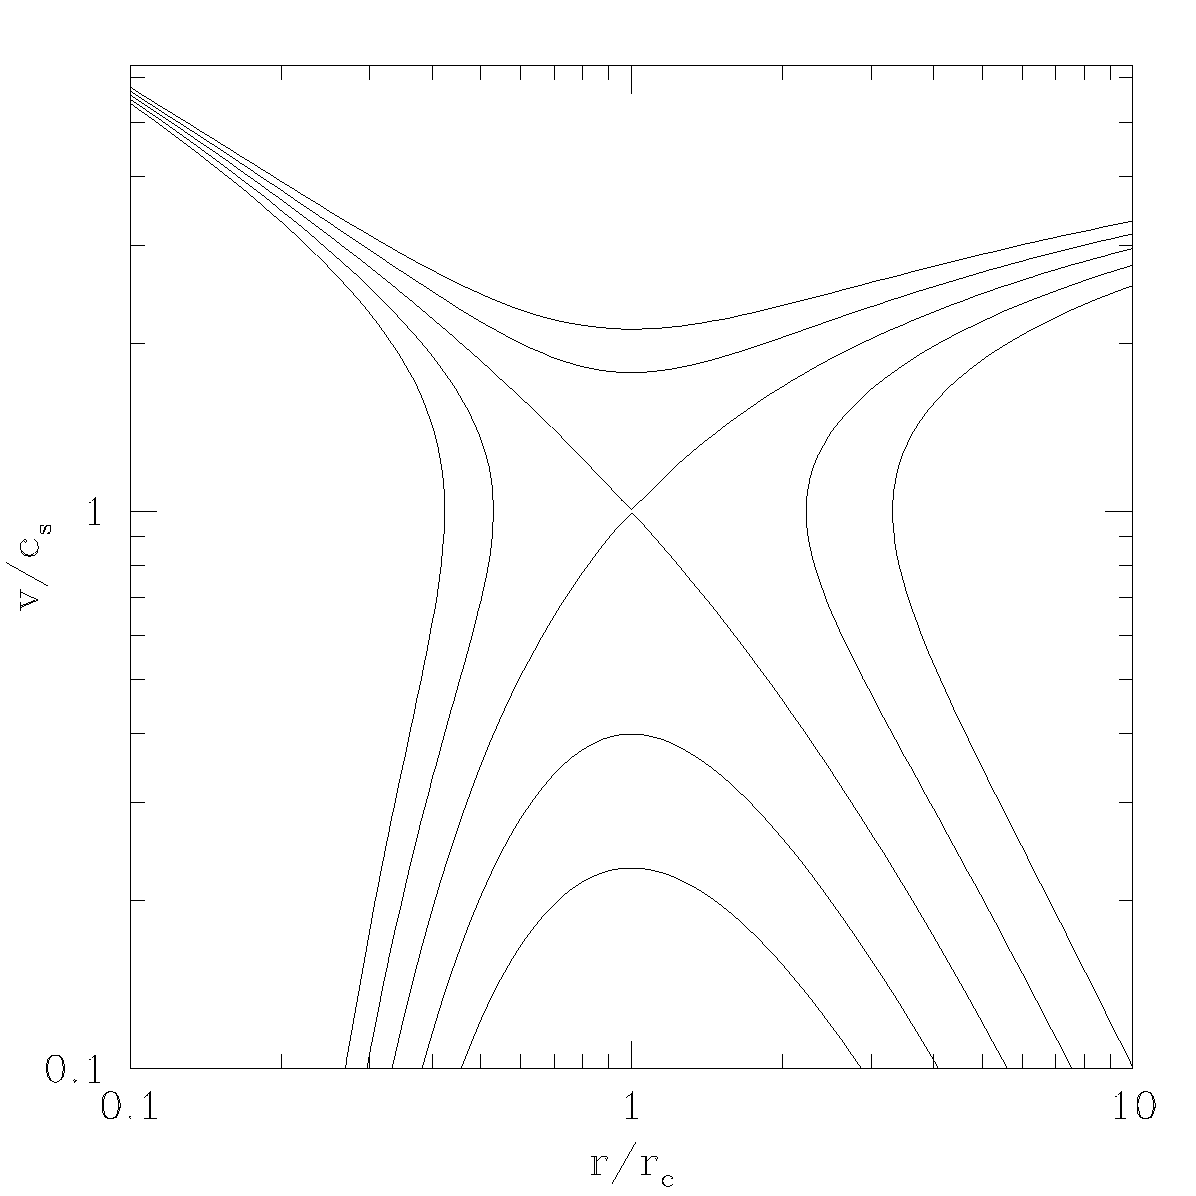
\includegraphics[width=\textwidth]{isothermal} 
\caption{The velocity structure for an isothermal wind, neglecting
  angular momentum and magnetic fields.}
\label{fig:isothermal}
\end{figure}
}

\section{Problems}
\begin{enumerate}


\item{\bf Exact Solutions}

For which values of $\gamma$ can the Bernoulli equation
(Eq.~\ref{eq:725}) be solved using elementary methods (linear,
quadratic and cubic equations of the form in Eq.~\ref{eq:676}).  There
are many, however only a few have $1< \gamma < 5/3$.

\item{\bf Monoatomic Gas}

For a monoatomic gas, the value of $\gamma$ is $5/3$.  According
Eq.~\ref{eq:729}, the density at the critical radius is infinite, and
the critical radius itself goes to zero.  Explain how accretion from
atomic gas would proceed.

\item{\bf Accretion Disk}

  Calculate the surface temperature of the accretion disk as a
  function of radius, central mass and accretion rate.  You may assume
  that all of the energy generated by viscous stresses is radiated
  locally as blackbody emission.  Calculate the cumulative amount of
  flux as a function of temperature.  Does most of the radiation
  emerge from regions at high temperature, at low temperatures or
  somewhere in between?

\item{\bf Bondi Solution}

Generate a picture like Fig.~\ref{fig:bondi} for the Bondi
solution to spherical accretion.  Use $\gamma=9/7$.

\item{\bf Bondi Solution --- Harder}

Generate a Fig.~\ref{fig:bondi} for the Bondi
solution to spherical accretion.  Use $\gamma=7/5$.

\item{\bf Accretion Energetics}

\begin{enumerate}
\item Let's use Newtonian gravity for simplicity here. How much
  kinetic energy does a gram of material have if it falls freely from
  infinity to the surface of a star of mass $M$ and radius $R$?
\item How much energy is released if a gram of material falls from a
  circular orbit just above the stellar surface onto the stellar
  surface? To put it another way, what is the kinetic energy of the
  material in the circular orbit?
\item Hydrogen burning releases about $6 \times 10^{18}$~erg/g. How does
  accretion of hydrogen onto a neutron star ($R=10$~km, $M=1.4 \mathrm{M}_\odot$) differ
  from accretion onto a white dwarf ($R=10000$~km, $M=0.6 \mathrm{M}_\odot$)?
\item What is the total about of energy released per gram of material
  as it falls from infinity to the surface of a neutron star? How many
  grams of material would have to fall each second on the neutron star
  to generate an Eddington luminosity through accretion? This is
  called the Eddington accretion rate.
\end{enumerate}

\item{ \bf A Simplified Accretion Disk }
This is a simplified model for an accretion disk. It is simpler than
the model outlined in the chapter but it will give the
right order of magnitude for things. We are also using Newtonian
gravity.
\begin{enumerate}
\item Let's divide the accretion disk into a series of rings each of
  mass $dm$. What is the total energy of a ring at a distance r from
  the central black hole of mass $M$?

\item Let's say that the ring shrinks by a distance $dr$. What is the
  change in the energy of the ring ($dE/dr$)?  As the ring shrinks mass
  is moving toward the black hole. Divide both sides the answer to (b)
  by $dt$ to get an equation for the energy loss rate per radial
  interval.

\item What is the energy loss rate per unit area?

\item Let's assume that this energy is radiated at the radius where it
  is liberated. Using the blackbody formula what is the temperature of
  the surface of the disk?

\item Let's assume that the disk extends from an outer radius $r_A$ to
  an inner radius $r_0$. What is the total luminosity of the disk if
  the accretion rate is $dm/dt$? What and where is the peak
  temperature of the disk? What and where is the minimum temperature
  of the disk?

\item Sketch the spectrum from the accretion disk on a log-log
  plot. You can use temperature units for the energy axis (i.e. $kT_\mathrm{max}$
  and $kT_\mathrm{min}$). To do this you will have to think about the peak flux
  from a blackbody at a particular temperature and the size of the
  disk that radiates at $T_\mathrm{max}$ and $T_\mathrm{min}$.

\item The accretion rate is determined by the evolution of the orbit
  of the black hole with its companion, so it doesn't know about the
  Eddington limit of the black hole. What do you suppose happens if
  the rate that matter falls onto the disk exceeds the Eddington
  limit?

\item What major bit of physics has been left out of this analysis?
\end{enumerate}
\end{enumerate}
%%% Local Variables:
%%% TeX-master: "book"
%%% End:
